\section{Datenübertragung}
\label{sec:Daten}
Im folgenden wird ein Konzept beschrieben, um Daten des VARAN-Buses optisch und bidirektional zu übertragen. Ausserdem wird eine Sende- und Empfängerschaltung entworfen, um einen Teilbereich des Konzepts zu überprüfen und wichtige Erkenntnisse für die Fortsetzung der Arbeit zu sammeln.  
\subsection{Konzept}
In Abbildung \ref{fig:Konzept_Daten} wird grob das Konzept zur optischen Datenübertragung gezeigt.

\begin{figure}[h]
	\centering
	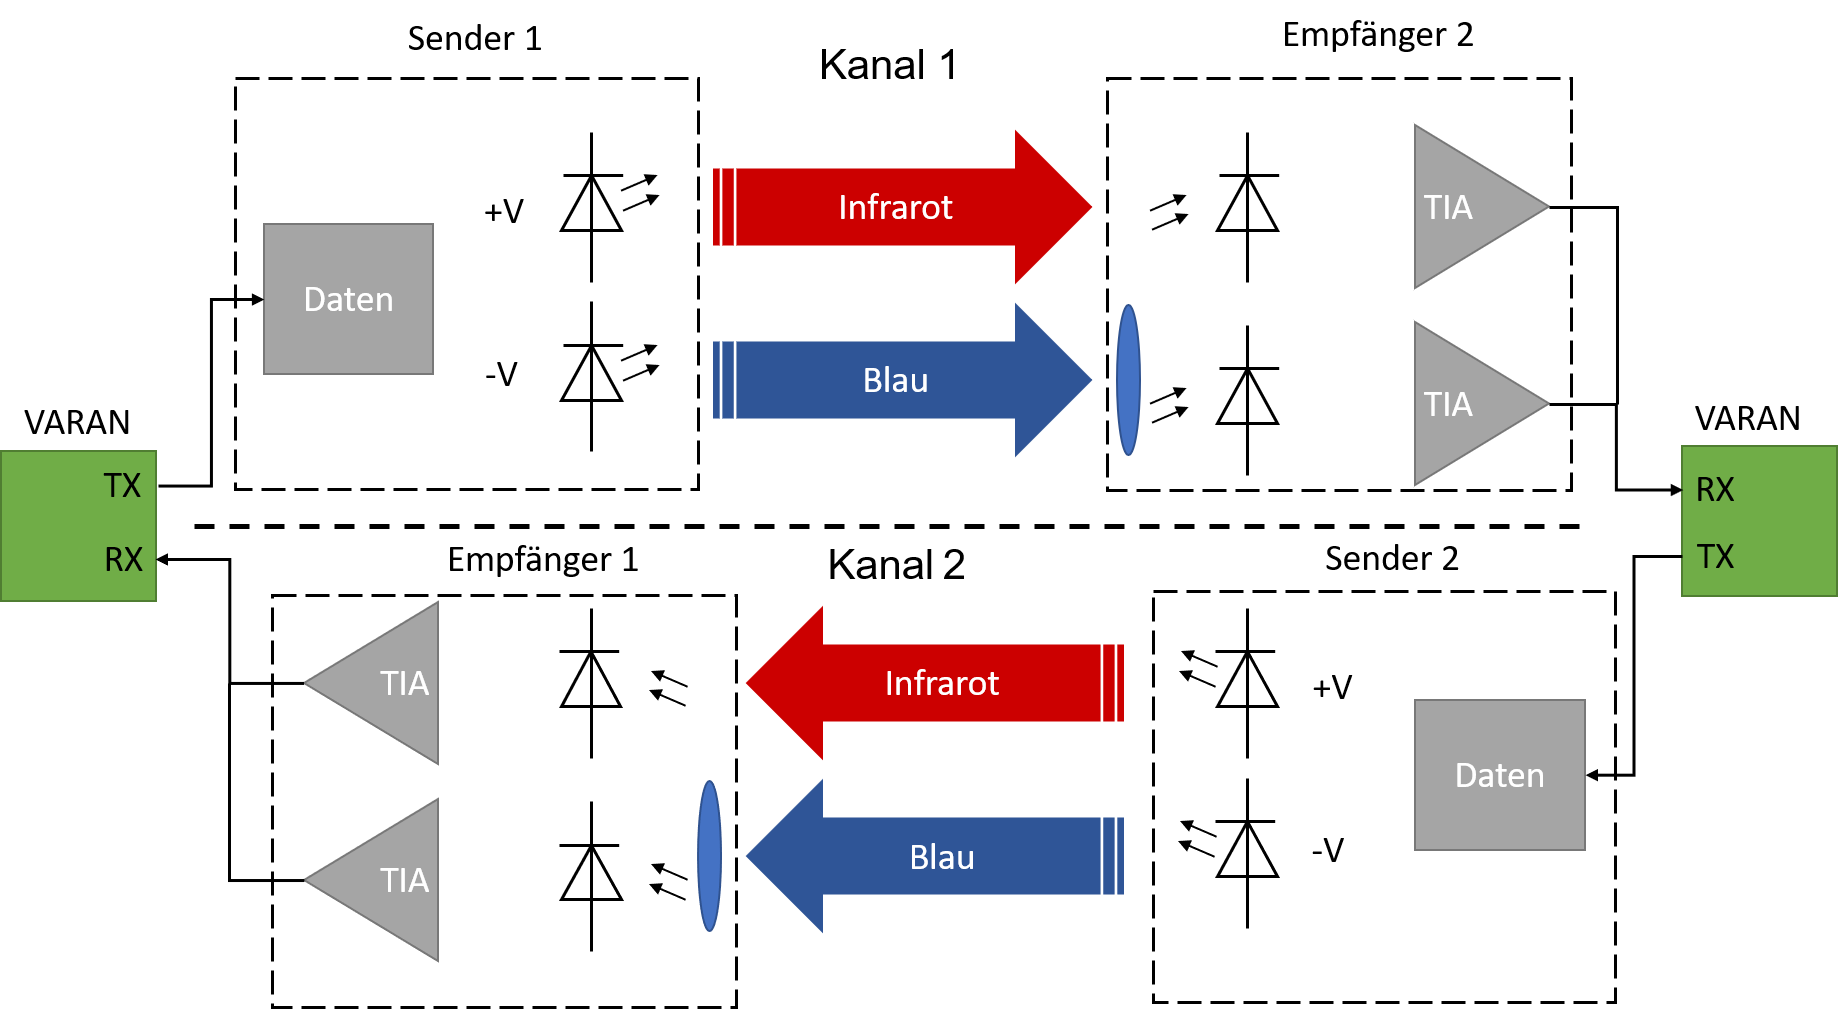
\includegraphics[width=\linewidth]{Konzept_Daten.png}
	\caption{Konzept der optischen Datenübertragung}\label{fig:Konzept_Daten}
\end{figure}

In der Abbildung sind die beiden Kanäle zu erkennen, welche optisch voneinander getrennt sind. Jeder Kanal überträgt dabei die Daten nur in jeweils eine Richtung. Beide Kanäle zusammen sorgen für die gewünschte Bidirektionalität. Auf der Primär- und Sekundärseite hat es jeweils eine Sende- und Empfangseinheit. Eine Sendeeinheit besteht aus der Datenerfassung und den Leuchtdioden. Da der VARAN-Bus MLT-3 codiert ist, müssen drei Zustände übertragen werden können. Die positiven Spannungspegel werden mit einer Infrarot-LED übertragen und die negativen Spannungspegel mit einer blauen LED. Der Zustand \glqq0\grqq steht an, wenn keine der LEDs leuchtet.
\newline
Eine Empfangseinheit besteht aus Photodioden und Verstärkerschaltungen. Im blauen Spektralbereich werden mit Hilfe eines optischen Filters vor der Photodiode die unerwünschten Spektralanteile herausgefiltert.
\newline Die beiden Sende- und Empfangseinheiten sind identisch aufgebaut und unterscheiden sich nur in der Übertragungsrichtung.

\paragraph{Sender}
In folgender Abbildung ist das Konzept einer Sendeeinheit detaillierter dargestellt.

\begin{figure}[h]
	\centering
	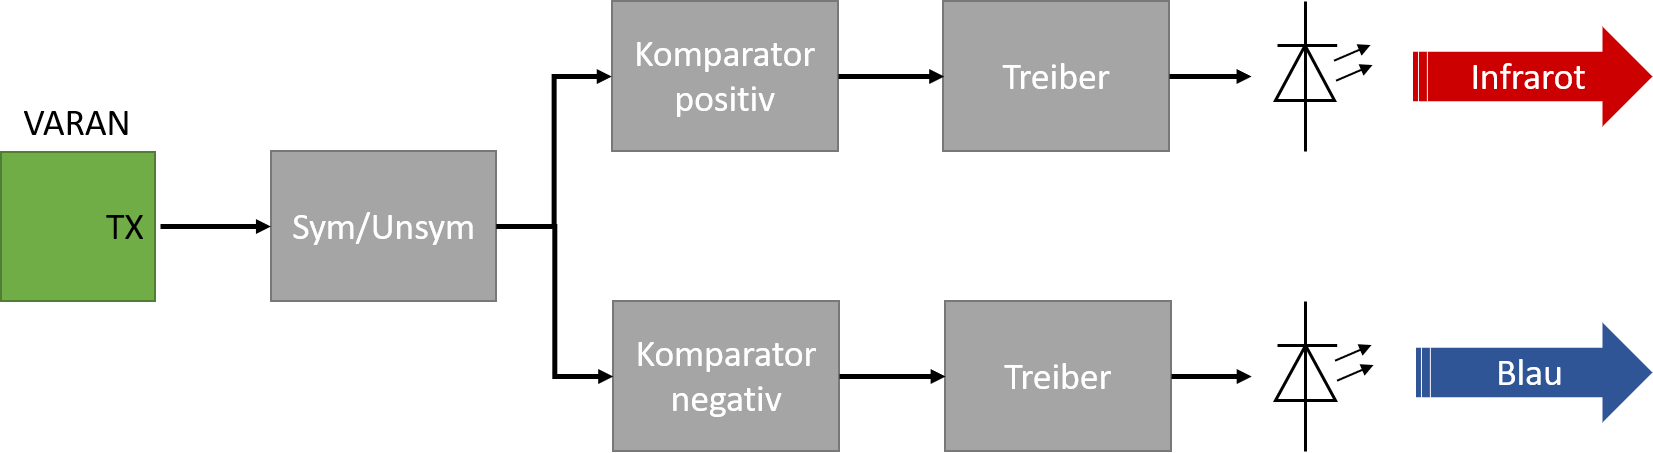
\includegraphics[width=\linewidth]{Konzept_Sender.png}
	\caption{Konzept der optischen Sendeeinheit}\label{fig:Konzept_Sender}
\end{figure}

Aus dem symmetrischen Signal des VARAN-Buses wird zuerst ein unsymmetrisches Signal erzeugt. Dafür kann ein Signal-Transformator eingesetzt werden. Das Signal hat nun einen Bezug zur Masse der restlichen Schaltung. Mit zwei Komparatoren wird unterschieden, ob es sich um einen positiven oder negativen Pegel handelt. Dafür werden Komparatoren mit möglichst kurzer Verzögerungszeit und ausreichender Bandbreite verwendet. Die Komparatoren steuern anschliessend die entsprechenden Treiber an. Als Treiber dient ein FET-Treiber Baustein mit hoher Treiberspannung für schnelle Anstiegs- und Abfallzeiten. Die LED wird mit einem N-Kanal-FET nach Masse geschaltet. Die Schaltzeiten der LED sind entscheidend um auf die geforderte Schaltfrequenz von \textgreater \SI{30}{MHz} zu kommen. Dafür wurde einerseits ein FET mit kleiner Gate-Kapazität gewählt und andererseits auf kurze Anstiegs- und Abfallzeiten der LED geachtet.
\newline
Mit einer kleinen Erweiterung der Beschaltung der LED können die Anstiegs- und Abfallzeiten nochmals reduziert werden. Folgende Abbildung zeigt die Ansteuerung der LED mitsamt der Erweiterung von $R_{2}$, $C$ und $L$.

 \begin{figure}[h]
 	\centering
 	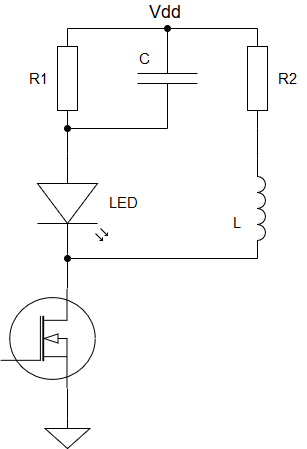
\includegraphics[width=0.3\linewidth]{Fast_LED.png}
 	\caption{Erweiterte Schaltung um Schaltzeiten zu verkürzen}\label{fig:Fast_LED}
 \end{figure}

Durch den Leckstrom des FET wird die LED auch im abgeschalteten Zustand mit einigen Ladungsträgern durchflossen, was die Anstiegszeit geringfügig verkürzt. Im Einschaltmoment sorgt der Kondensator $C$ für einen Kurzschluss und überbrückt den Vorwiderstand $R_{1}$. Es kommt zu einem Strompeak, der die Kapazität der LED schneller laden lässt. Die Anstiegszeit wird dadurch massiv verkürzt. Im Ausschaltmoment induziert das Magnetfeld in der Spule $L$ eine negative Spannung. Folglich werden die Ladungsträger aus der LED gezogen. Dadurch wird auch die Abfallzeit gegenüber dem \glqq einfachen\grqq Ausschalten verkürzt.

\paragraph{Empfänger}
In folgender Abbildung wird das Konzept einer Empfangseinheit detaillierter dargestellt.

\begin{figure}[h]
	\centering
	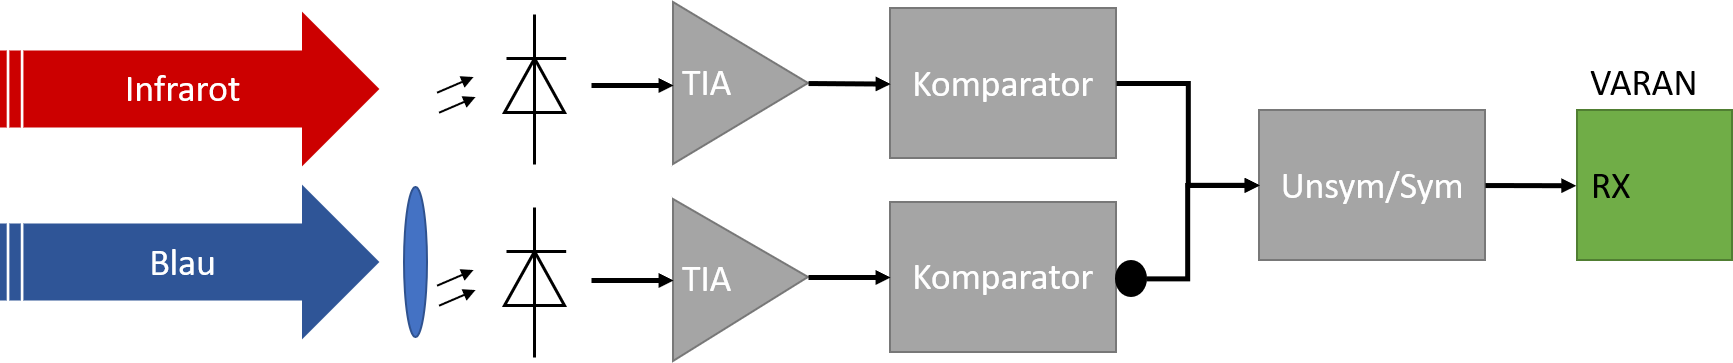
\includegraphics[width=\linewidth]{Konzept_Empfaenger.png}
	\caption{Konzept der optischen Empfangseinheit}\label{fig:Konzept_Empfaenger}
\end{figure}

Der von der Photodiode erzeugte Strom wird mit einer Transimpedanzverstärkerschaltung in eine Spannung gewandelt und verstärkt. Wie im Kapitel \nameref{sec:Grundlagen} bereits erwähnt, ist eine hohe Bandbreite bei der Verstärkerschaltung erforderlich. Deshalb ist ein Verstärker mit hohem Gain-Bandwidth Product und kleiner Eingangskapazität zu wählen. Auch die parasitäre Kapazität der Photodiode beeinflusst die Bandbreite, weshalb auch diese möglichst klein gewählt werden muss. Durch negative Biasspannung an der Anode kann die Kapazität nochmals reduziert werden.
\newline
Nach dem Transimpedanzverstärker werden mit Komparatoren die Pegel in Amplitude und Form angepasst. Das Signal vom blauen Spektralbereich, welches die negativen Pegel überträgt wird noch invertiert. Mit einem Signal-Transformator wird aus dem unsymmetrischen Signal wieder ein symmetrisches Signal generiert und dieses zurück an den VARAN-Bus geführt.

\paragraph{Kanal}
Da die optische Übertragung auf einer drehbaren Konstruktion stattfindet, ist keine direkte Verbindung sichergestellt. Deshalb bestehen die beiden Kanäle aus einem lichtstreuenden Werkstoff und sind optisch voneinander isoliert. Nachfolgende Abbildung zeigt den prinzipiellen Aufbau der Kanäle.

\begin{figure}[h]
	\centering
	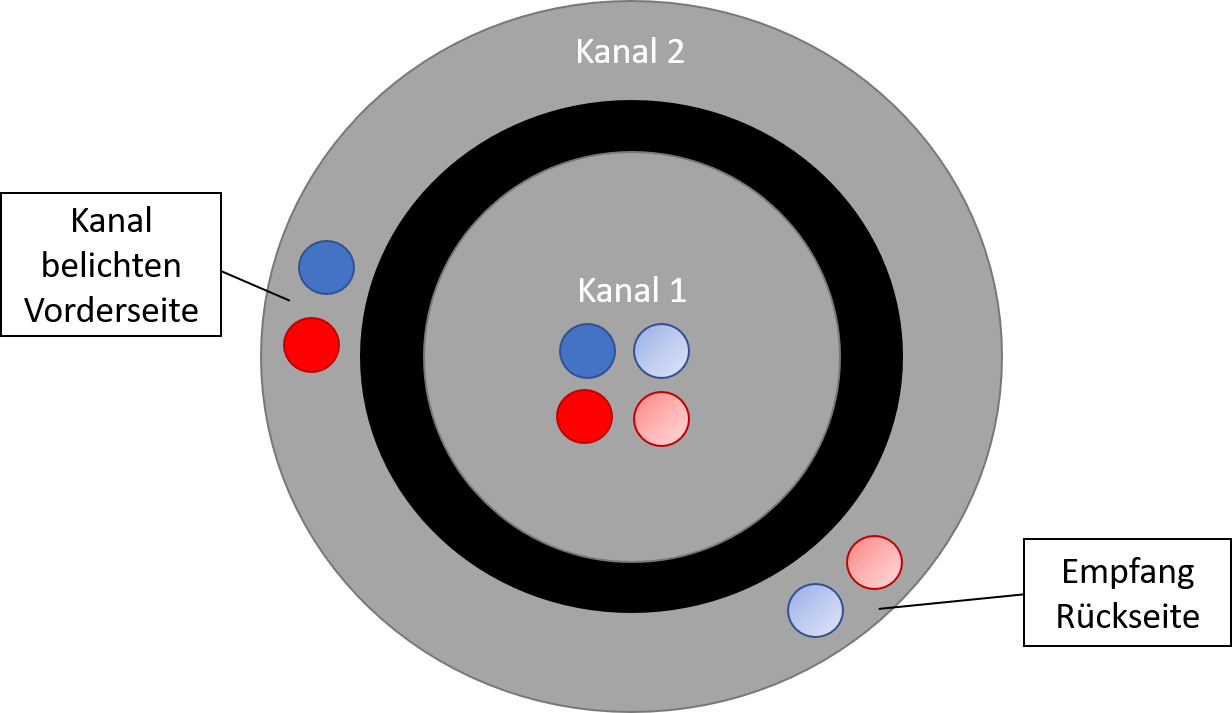
\includegraphics[width=0.6\linewidth]{Konzept_Kanal.png}
	\caption{Konzept der Kanäle}\label{fig:Konzept_Kanal}
\end{figure}

In der Abbildung ist die optische Isolation (schwarz) gut zu erkennen, welche die gegenseitige Störung zwischen den Kanälen verhindert. Im Kanal 1 ist die Rotation der mechanischen Konstruktion unproblematisch, da sich Sender und Empfänger auf der Drehachse befinden. Der Kanal 2 nimmt das Licht auf der einen Seite auf und der lichtstreuende Werkstoff (grau) verteilt es im ganzen Kreisring. Nun spielt es auf der Empfängerseite keine Rolle mehr, in welchem Abschnitt auf dem Kreisring man sich befindet.

\subsection{Dimensionierung Testaufbau}
Um wichtige Erkenntnisse für den weiteren Projektverlauf zu gewinnen, wurde ein Testaufbau realisiert. Dieser beinhaltet eine Sende- und Empfangseinheit um einen Rechteckpuls im Infrarotbereich zu übertragen. 
In diesem Unterkapitel wird auf die wichtigsten Punkte zur Dimensionierung des Testaufbaus eingegangen.
\paragraph{Sender} 
Als Eingang beim Sender dient eine BNC-Buchse, um den Rechteckpuls einzuspeisen. Als Gatetreiber des FET wird der ISL55110 vom Hersteller Renesas verwendet. Dieser zeichnet sich durch kurze Anstiegs- und Fallzeiten von \SI{1.5}{ns} bei einer Last von \SI{100}{pF} aus.
Der gewählte N-Kanal-FET ist ein BSS316N vom Hersteller Infineon. Durch die kleine Eingangskapazität von \textless \SI{100}{pF} kann der FET in Kombination mit dem Gatetreiber sehr schnell geschaltet werden.
Als Infrarot-Emitter wurde die SFH4235 von OSRAM gewählt. Die Leuchtdiode kann mit Anstiegs- und Abfallzeiten von 7/\SI{14}{ns} mit \textgreater \SI{30}{MHz} betrieben werden und ist deshalb für diese Anwendung geeignet. Folgende Abbildung zeigt das Spektrum des Infrarot-Emitters.

\begin{figure}[h]
	\centering
	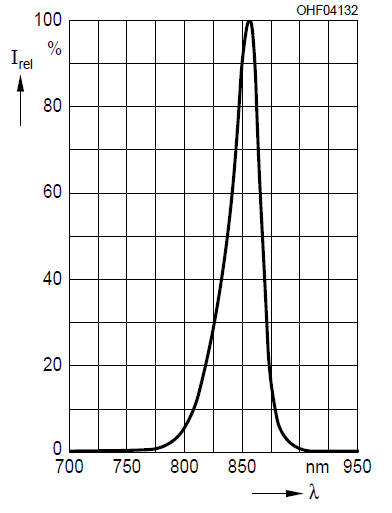
\includegraphics[width=0.4\linewidth]{Spektrum_Infra.png}
	\caption{Spektrum SFH4235}\label{fig:Spektrum_Infra}
\end{figure}

Wie in der Abbildung zu erkennen ist, hat das Spektrum den Peak bei \SI{860}{nm}. Die Photodiode auf der Empfängerseite muss dementsprechend passend zum Spektrum ausgewählt werden. Die im Konzept beschriebene Schaltungsergänzung wurde im Testaufbau vorbereitet. Weil die Standartbeschaltung schnell genug ist, wird die Ergänzung jedoch nicht bestückt.

\paragraph{Empfänger}
Mit zwei Z-Dioden (SZBZX84C3V3 und BZD27C13) und einem Operationsverstärker (LM7321) als Buffer geschaltet, wird eine Speisung für die Empfängerschaltung generiert. Diese liefert die benötigten Spannungen von \SI{3.3}{V} für die integrierten Bauteile und \SI{-13}{V} um die Photodiode mit einer negativen Biasspannung vorzuspannen. Die Beschaltung ist im Schema im Anhang abgebildet.
\newline
Es wurden zuerst drei verschiedene Photodioden ausgewählt und ausgemessen.


\subsection{Simulation}
Im Simulations-Abschnitt wird die Dimensionierung und das Konzept überprüft.
\subsection{Testaufbau}
In diesem Unterkapitel wird der Testaufbau beschrieben.